\subsection{Benutzerschnittstelle}

\begin{center}
\setlength\fboxsep{20pt}
\setlength\fboxrule{1pt}
\fbox{
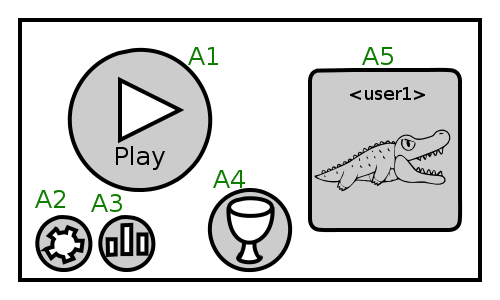
\includegraphics[scale=0.5]{Systemmodelle/images/main_menu.png}
}
\captionof{figure}{Hauptmenü}
\end{center}

\subsubsection{Hauptmenü}
Wird beim Neustarten der App als Erstes geöffnet. Wird die App zum Ersten mal verwendet, oder existieren keine Profile, wird zunächst die Profilerstellung (Teil 1) geöffnet.
\begin{requirements}
\req{B1} Öffnet die Levelübersicht.
\req{B2} Öffnet das Einstellungsmenü.
\req{B3} Öffnet die Statistiken. Übernimmt den aktuellen Benutzer als ausgewählten Benutzer in der Statistik.
\req{B4} Öffnet die Achievements.
\req{B5} Öffnet die Profilauswahl.
\end{requirements}

\begin{center}
\setlength\fboxsep{20pt}
\setlength\fboxrule{1pt}
\fbox{
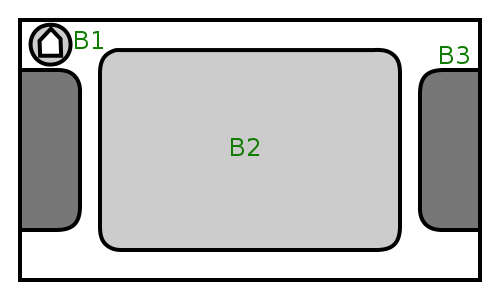
\includegraphics[scale=0.5]{Systemmodelle/images/level_overview.png}
}
\captionof{figure}{Levelübersicht}
\end{center}

\subsubsection{Levelübersicht}
\begin{requirements}
\req{B1} Navigiert zurück zum Hauptmenü.
\req{B2} Ein Levelblock. Repräsentiert eine bestimmte Anzahl und/oder Kategorie von elementaren Leveln. Der Sandbox-Modus wird durch einen Levelblock repräsentiert. Öffnet die Leveldetailübersicht.
\req{B3} Der in der Levelanordnung nächste Levelblock. Wird durch eine "Swipe"-Eingabe zentriert und nimmt so den Platz des aktuellen Levelblocks ein.
\end{requirements}

\begin{center}
\setlength\fboxsep{20pt}
\setlength\fboxrule{1pt}
\fbox{
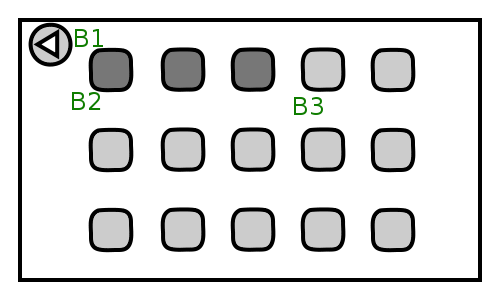
\includegraphics[scale=0.5]{Systemmodelle/images/level_overview_detail.png}
}
\captionof{figure}{Leveldetailübersicht}
\end{center}

\subsubsection{Leveldetailübersicht}
\begin{requirements}
\req{B1} Navigiert zurück zur Levelübersicht.
\req{B2} Ein verfügbares Level. Startet das jeweilige Level.
\req{B3} Ein nicht verfügbares Level. Kann durch erfolgreiches Lösen der vorhergehenden Level freigeschaltet werden und wird dann verfügbar.
\end{requirements}

\begin{center}
\setlength\fboxsep{20pt}
\setlength\fboxrule{1pt}
\fbox{
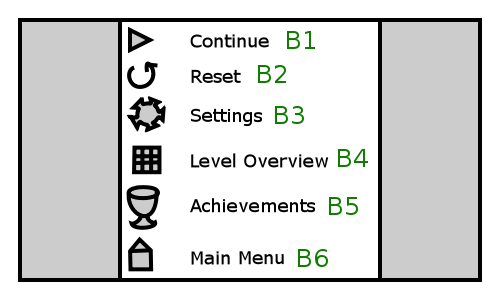
\includegraphics[scale=0.5]{Systemmodelle/images/ingame_menu.png}
}
\captionof{figure}{Spielmenü}
\end{center}

\subsubsection{Spielmenü}
\begin{requirements}
\req{B1} Wechselt zurück zum laufenden Level.
\req{B2} Öffnet das Level im Startzustand. Verwirft den aktuellen Zustand des Levels.
\req{B3} Öffnet das Einstellungsmenü.
\req{B4} Navigiert zurück zur Leveldetailübersicht. Verwirft den aktuellen Zustand des laufenden Levels.
\req{B5} Öffnet die Achievements.
\req{B6} Navigiert zurück zum Hauptmenü. Verwirft den aktuellen Zustand des laufenden Levels.
\end{requirements}

\begin{center}
\setlength\fboxsep{20pt}
\setlength\fboxrule{1pt}
\fbox{
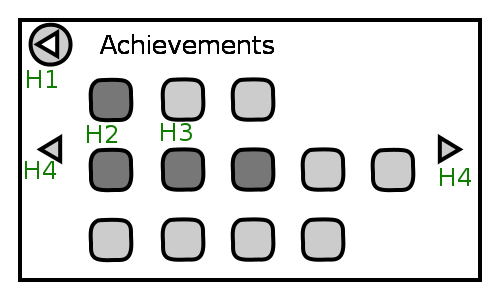
\includegraphics[scale=0.5]{Systemmodelle/images/achievements.png}
}
\captionof{figure}{Achievements}
\end{center}

\subsubsection{Achievements}
\begin{requirements}
\req{B1} Navigiert zurück zum vorigen Navigationpunkt (Spielmenü oder Hauptmenü).
\req{B2} Erreichtes Achievement. Öffnet die Detailansicht mit Icon und Beschreibung des angewählten Achievements.
\req{B3} Noch nicht erreichtes Achievement. Ist wahlweise ausgegraut oder unsichtbar. Öffnet, falls nicht unsichtbar, eine Beschreibung, wie das gewählte Achievement zu erreichen ist.
\req{B4} Navigiert zum vorigen/nächsten Achievementblock.
\end{requirements}

\begin{center}
\setlength\fboxsep{20pt}
\setlength\fboxrule{1pt}
\fbox{
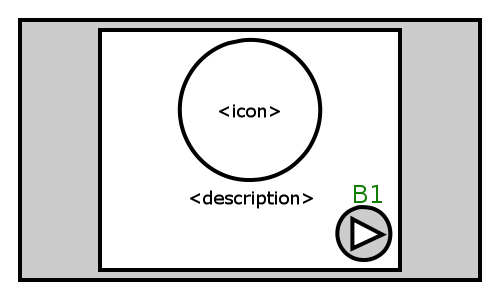
\includegraphics[scale=0.5]{Systemmodelle/images/achievement_notification.png}
}
\captionof{figure}{Achievement-Benachrichtigung}
\end{center}

\subsubsection{Achievement-Benachrichtigung}
Alle Achievement-Benachrichtigungen werden nach erfolgreichem Abschluss eines Levels angezeigt.
\begin{requirements}
\req{B1} Schließt die Benachrichtigung. Wurden weitere Achievements erreicht, erscheint die nächste Benachrichtigung, ansonsten wird mit dem üblichen Levelschema fortgefahren. 
\end{requirements} 

\begin{center}
\setlength\fboxsep{20pt}
\setlength\fboxrule{1pt}
\fbox{
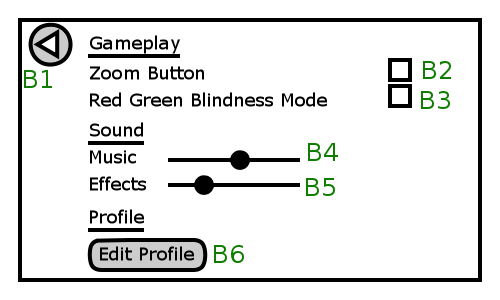
\includegraphics[scale=0.5]{Systemmodelle/images/settings.png}
}
\captionof{figure}{Einstellungsmenü}
\end{center}

\subsubsection{Einstellungsmenü}
\begin{requirements}
\req{B1} Navigiert zurück zum vorigen Navigationpunkt (Spielmenü oder Hauptmenü).
\req{B2} (De-)Aktiviert die buttongesteuerte Zoomfunktion im Level (statt dem üblichen Multitouch-Zoom).
\req{B3} (De-)Aktiviert den Rot-Grün-Schwäche-Modus.
\req{B4} Setzt die Musiklautstärke.
\req{B5} Setzt die Effektlautstärke.
\req{B6} Öffnet ein Menü mit den Optionen zum Bearbeiten des Profils (Name ändern/Profilbild ändern/Löschen).
\end{requirements}

\begin{center}
\setlength\fboxsep{20pt}
\setlength\fboxrule{1pt}
\fbox{
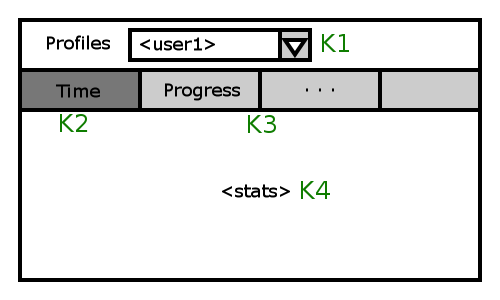
\includegraphics[scale=0.5]{Systemmodelle/images/stats.png}
}
\captionof{figure}{Statistiken}
\end{center}

\subsubsection{Statistiken}
\begin{requirements}
\req{B1} Aktuell ausgewählter Benutzer. Beim Öffnen der Statistiken ist der Benutzer gewählt, von dessen Profil aus die Statistiken geöffnet wurden. Öffnet ein Dropdownmenü zur Auswahl eines Benutzers.
\req{B2} Aktuell ausgewählter Tab.
\req{B3} Restliche thematische Tabs. Können durch Touch-Eingabe gewählt oder durch Swipe-Navigation erreicht werden. Tableiste kann je nach Anzahl der Tabs gescrollt werden.
\req{B4} Statistikeinträge. Sind durch Tableiste thematisch gruppiert. Können je nach Anzahl der Einträge gescrollt werden.
\end{requirements}

\begin{center}
\setlength\fboxsep{20pt}
\setlength\fboxrule{1pt}
\fbox{
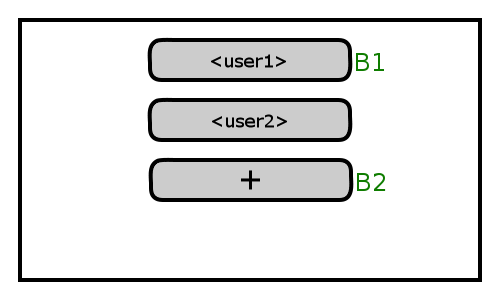
\includegraphics[scale=0.5]{Systemmodelle/images/change_user.png}
}
\captionof{figure}{Profilauswahl}
\end{center}

\subsubsection{Profilauswahl}
\begin{requirements}
\req{B1} Selektiert das gewählte Profil und öffnet dessen Hauptmenü.
\req{B2} Öffnet den Profilerstellungsdialog.
\end{requirements}

\begin{center}
\setlength\fboxsep{20pt}
\setlength\fboxrule{1pt}
\fbox{
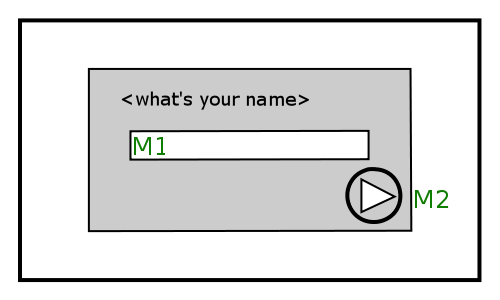
\includegraphics[scale=0.5]{Systemmodelle/images/profile_creator_1.png}
}
\captionof{figure}{Profilerstellung (Teil 1)}
\end{center}

\subsubsection{Profilerstellung(Teil 1)}
Wird bei erstmaliger Benutzung der App als Erstes geöffnet.
\begin{requirements}
\req{B1} Texteingabefeld für den Benutzernamen. Öffnet die Tastatur.
\req{B2} Bestätigt den eingegebenen Namen und fährt mit Profilerstellung (Teil 2) fort. Falls der eingegebene Name ungültig (z.B. leer) ist oder schon ein Profil mit diesem Benutzernamen existiert, wird eine entsprechende Meldung und eine Möglichkeit zur Änderung der Eingabe gegeben.
\end{requirements}

\begin{center}
\setlength\fboxsep{20pt}
\setlength\fboxrule{1pt}
\fbox{
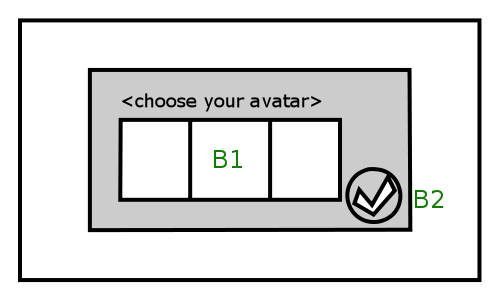
\includegraphics[scale=0.5]{Systemmodelle/images/profile_creator_2.png}
}
\captionof{figure}{Profilerstellung (Teil 2)}
\end{center}

\subsubsection{Profilerstellung(Teil 2)}
\begin{requirements}
\req{B1} Wahlmöglichkeiten für das Profilbild. Selektiert und markiert das gewählte Bild. Wird eventuell durch einen umfangreicheren Dialog ersetzt.
\req{B2} Bestätigt das ausgewählte Bild, erstellt ein Profil und öffnet dessen Hauptmenü.
\end{requirements}

